\documentclass{TIJMUjiaoanSY}
\pagestyle{empty}


\begin{document}


%课程名称
\kecheng{系统生物学}
%实验名称
\shiyan{实验三\ RNA-Seq测序数据的处理}
%教师姓名
\jiaoshi{伊现富}
%职称
\zhicheng{讲师}
%教学日期(格式:XXXX年XX月XX日XX时-XX时)
\riqi{2017年3月22日13:30-16:30}
%授课对象(格式:XXX系XXXX年级XX班(硕/本/专科))
\duixiang{生物医学工程与技术学院2014级生信班(本)}
%实验人数
\renshu{30}
%实验类型
\leixing{验证型}
%实验分组
\fenzu{一人一机}
%学时数
\xueshi{3}
%教材版本
\jiaocai{系统生物学实验讲义(自编教材)}


%教案首页
\firstHeader
\maketitle
\thispagestyle{empty}

\mudi{
\begin{itemize}
  \item 掌握RNA-Seq测序数据的分析流程。
  \item 熟悉Tuxedo套装的使用方法。
  \item 熟悉Galaxy的使用方法。
  \item 了解存储注释信息的GTF/GFF格式。
\end{itemize}
}

\fenpei{
\begin{itemize}
  \item (10')分析流程:回顾RNA-Seq测序数据分析的基本流程。
  \item (10')Tuxedo套装:回顾Tuxedo套装的组件及各自的作用。
  \item (10')GTF/GFF格式:回顾存储注释信息的GTF/GFF格式。
  \item (120')实验操作:从双端测序的RNA-Seq测序数据中寻找差异表达基因。
\end{itemize}
}

\cailiao{
\begin{itemize}
  \item 实验材料:以FASTQ格式存储的双端RNA-Seq测序数据。
  \item 主要仪器:联网的计算机。
  \item 分析工具:Galaxy,Tuxedo套装。
\end{itemize}
}

\zhongdian{
\begin{itemize}
  \item 难点:GTF/GFF格式;解决策略:通过实例进行讲解。
  \item 重点:Tuxedo套装的使用;解决策略:根据资料进行学习,通过练习熟练掌握。
\end{itemize}
}

\sikao{
\begin{itemize}
  \item 总结RNA-Seq测序数据的分析流程。
  \item 列举Tuxedo套装的组件并解释各自的作用。
  \item 解释存储注释信息的GTF/GFF格式。
\end{itemize}
}

\cankao{
\begin{itemize}
  \item Tuxedo套装
  \item Galaxy
\end{itemize}
}

\firstTail


%教案续页
\newpage
\otherHeader

\noindent
\begin{enumerate}
  \item 分析流程(10分钟)
    \begin{figure}[ht]
      \centering
      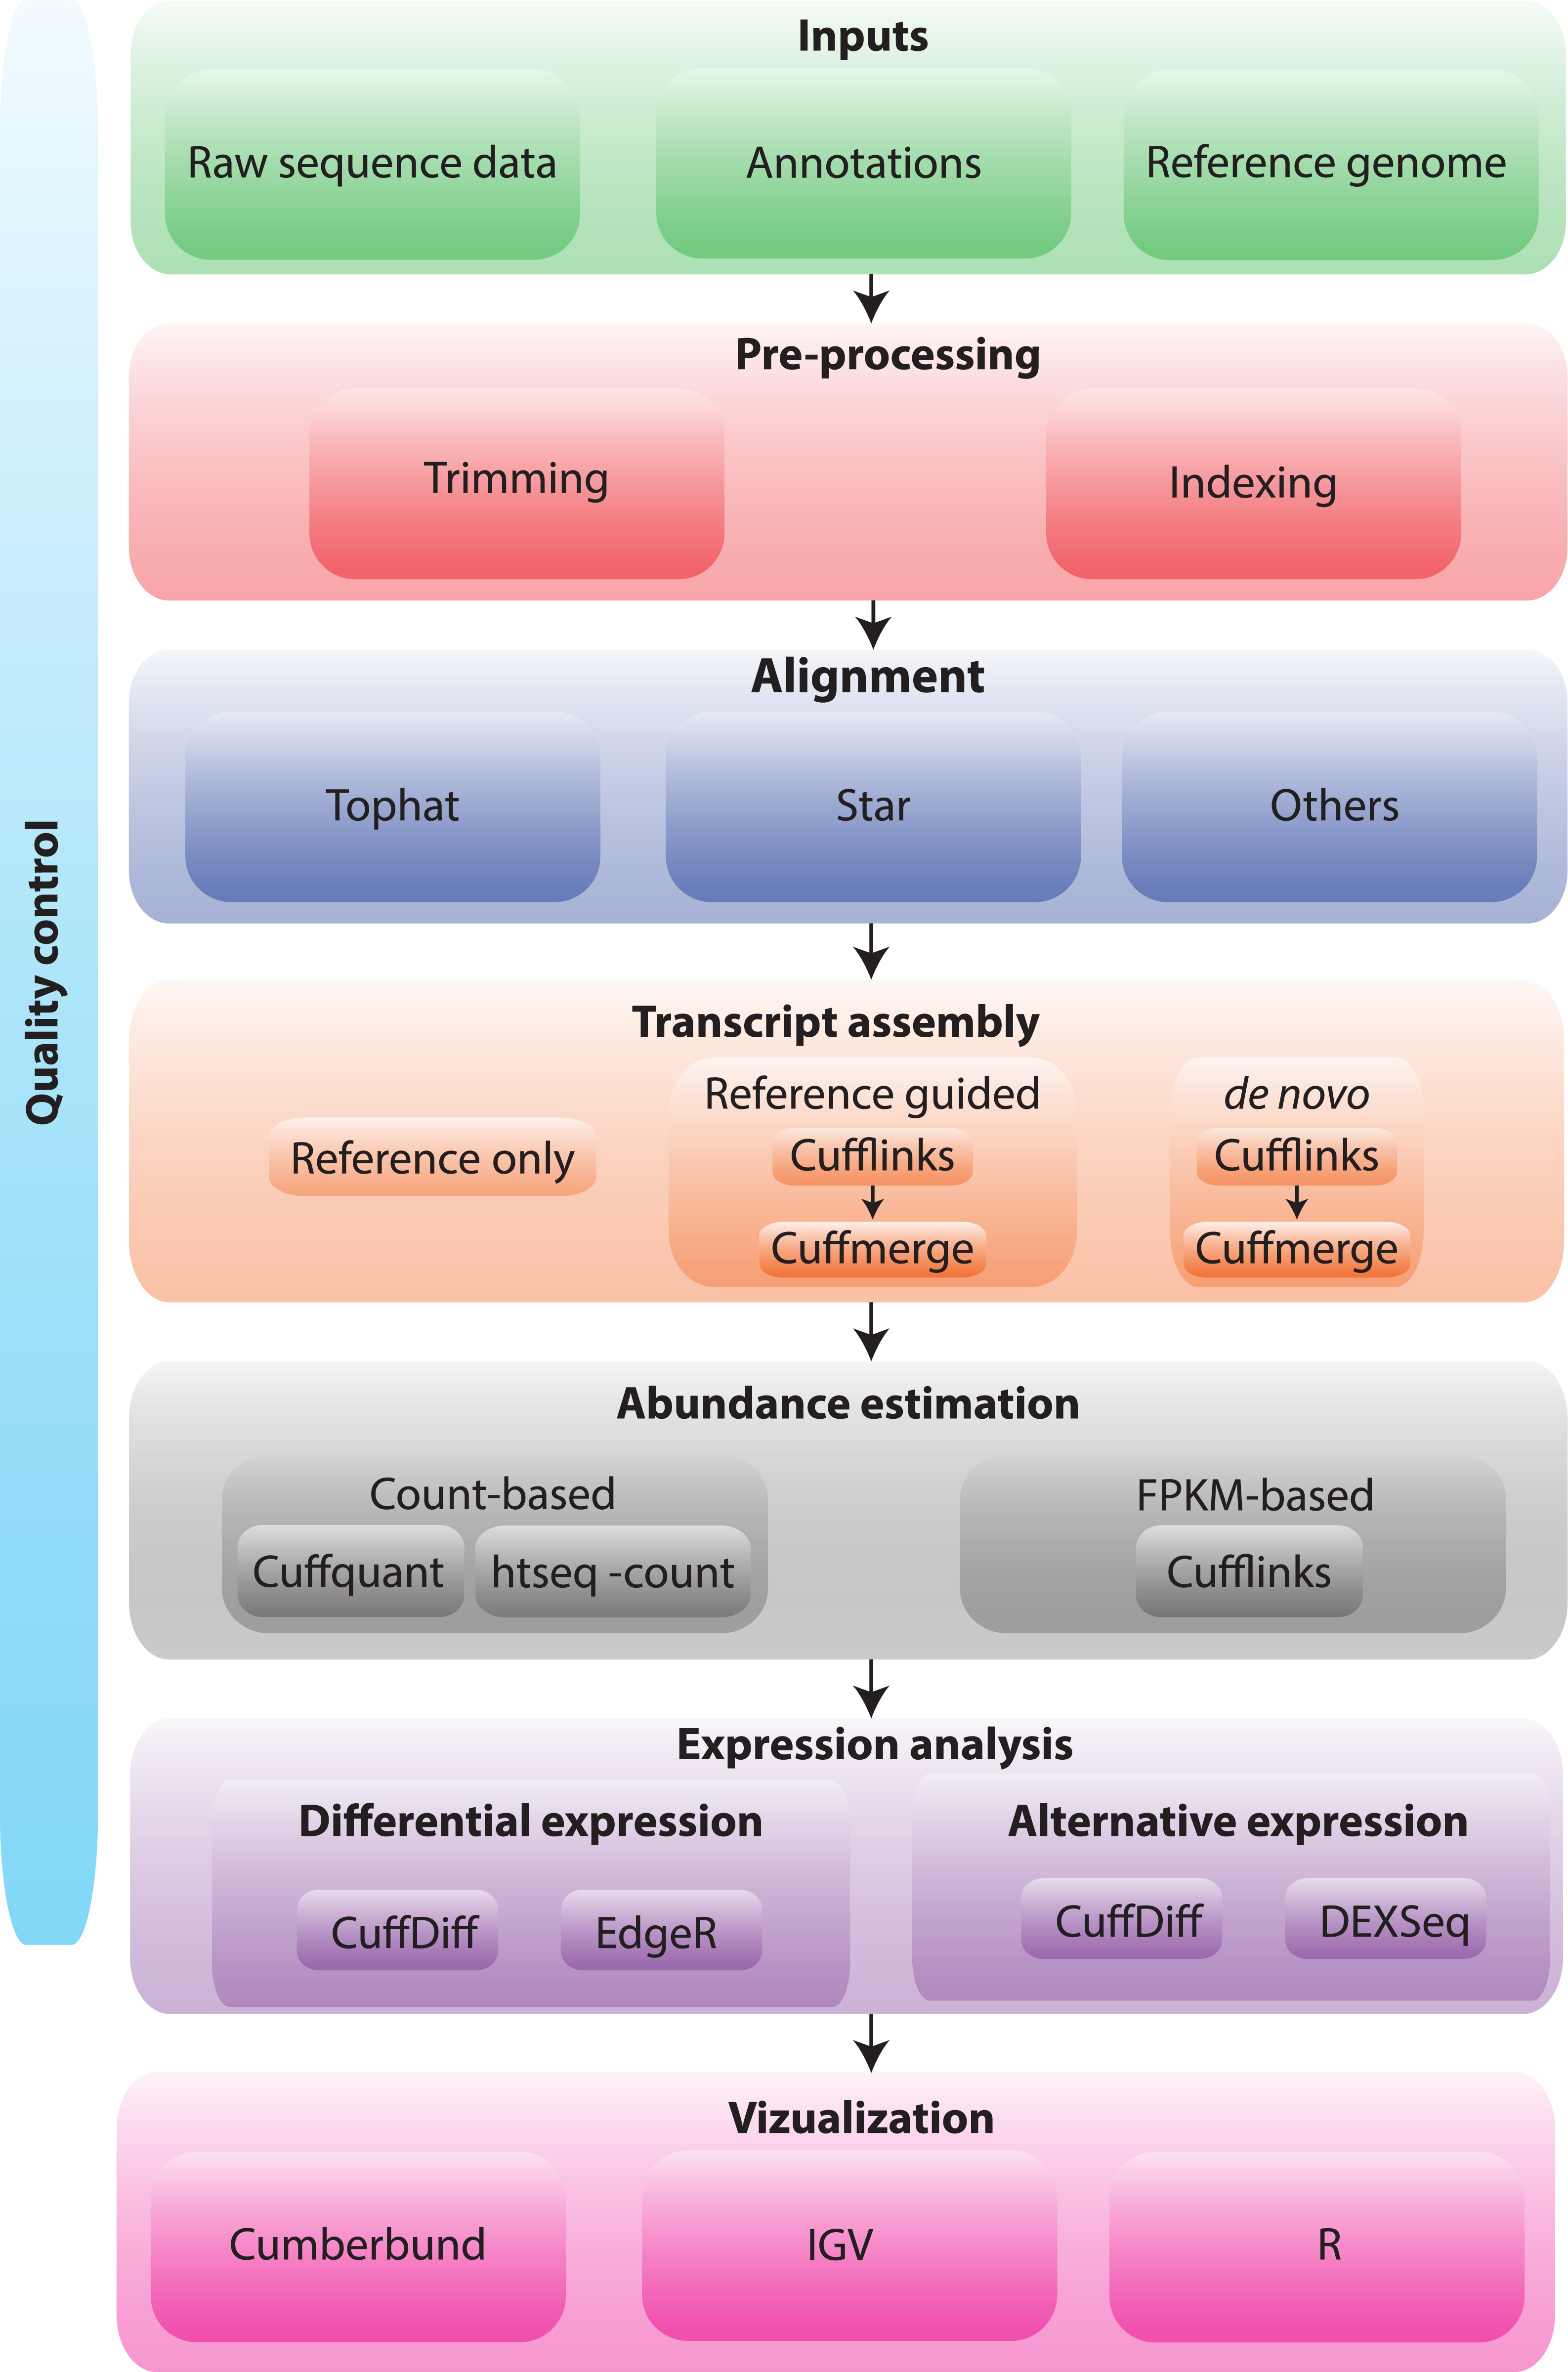
\includegraphics[width=0.35\textwidth]{c3_workflow_bx_05.png}
      \hspace{2em}
      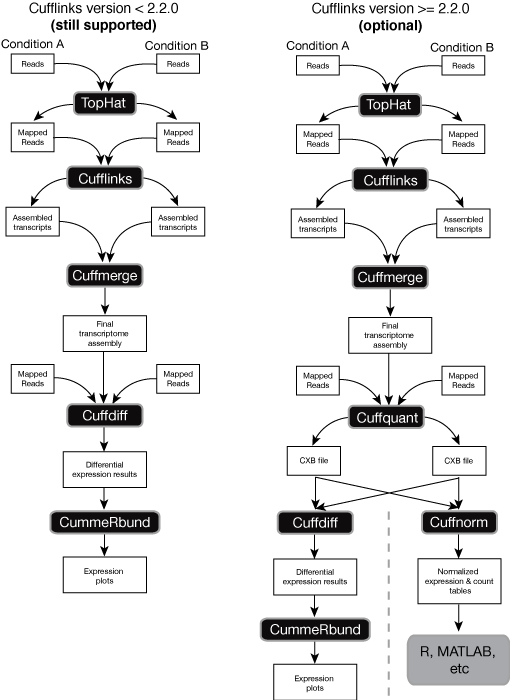
\includegraphics[width=0.38\textwidth]{c3_tool_tc_01.png}
    \end{figure}

  \item Tuxedo套装(10分钟)
% \parpic[fr]{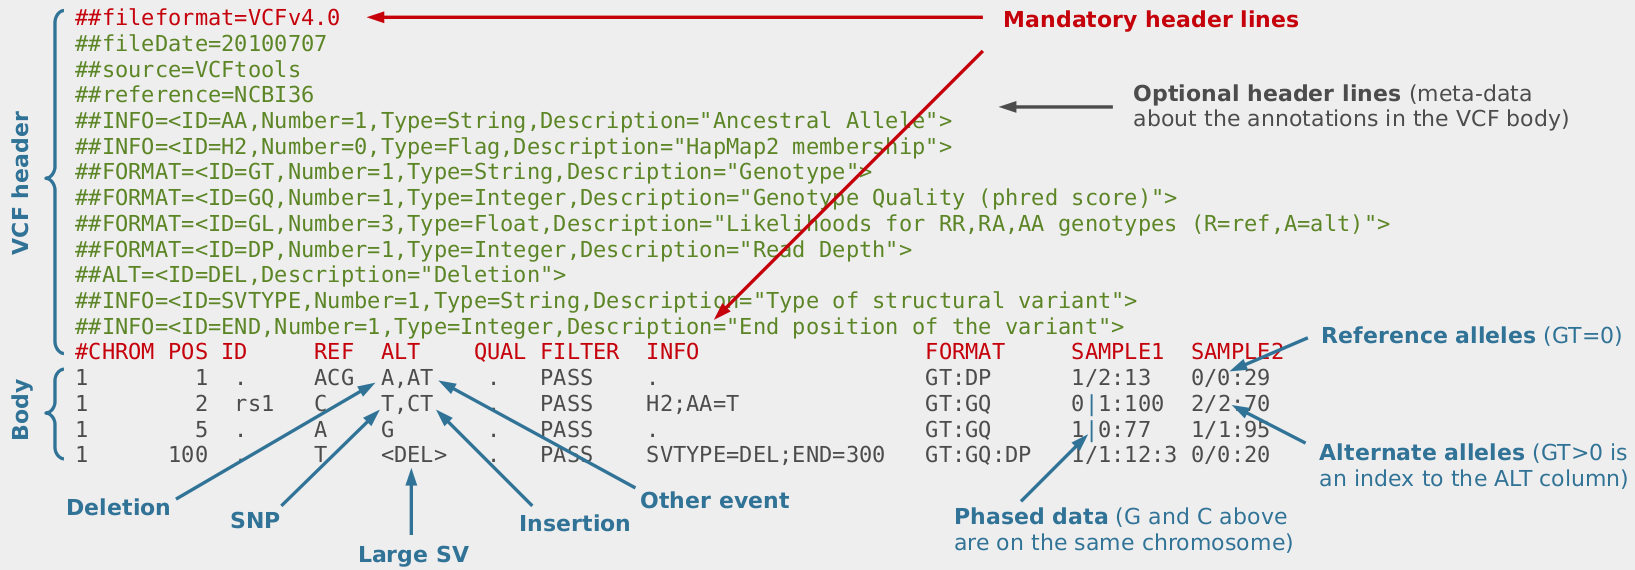
\includegraphics[width=11cm,height=6cm]{c2_format_vcf_05.png}}
    \begin{figure}[ht]
      \centering
      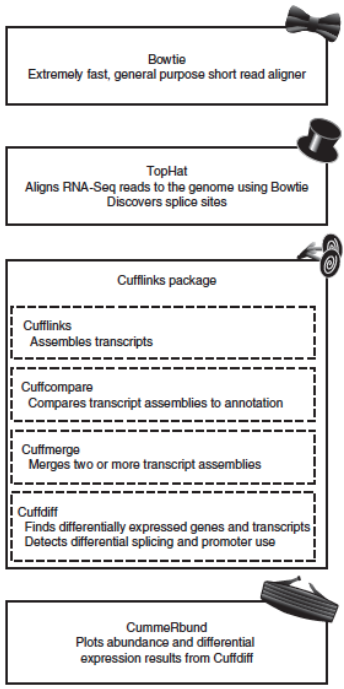
\includegraphics[width=0.22\textwidth]{c3_tool_tc_00.png}
      \hspace{2em}
      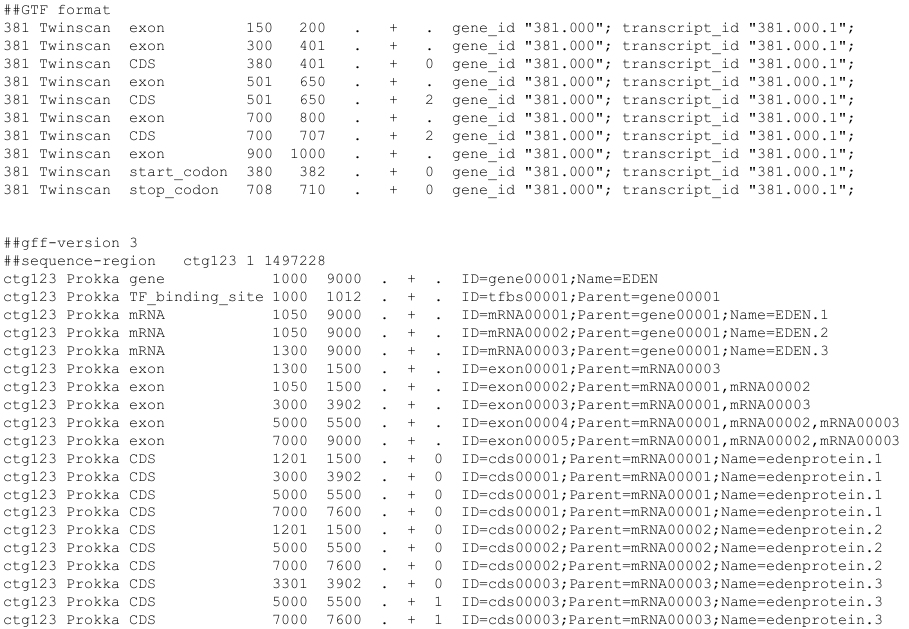
\includegraphics[width=0.61\textwidth]{c2_format_gtf_gff_03.png}
    \end{figure}

  \item GTF/GFF格式(10分钟)

  \item 实验操作(120分钟)
    \begin{enumerate}
      \item Upload data to Galaxy\textcolor{red}{(比较导入数据的不同方法;注意参数的设定)}
      \item Checking read quality with FastQC; Preprocessing\textcolor{red}{(参照实验一)}
      \item Map with TopHat\textcolor{red}{(尝试不同的参数设置;理解输出结果的含义)}
      \item Assemble and analyze transcripts\textcolor{red}{(理解参数和输出的含义)}
      \item Identify transcripts that are differentially expressed\textcolor{red}{(理解参数和输出的含义)}
      \item Visualization with CummeRbund\textcolor{red}{(尝试不同类型的可视化)}
    \end{enumerate}
\end{enumerate}


\otherTail


\end{document}

